
\documentclass[aspectratio=169]{beamer}
\usetheme{Boadilla}

\usepackage{qrcode}

\usepackage[utf8]{inputenc}       % Codificação de entrada
\usepackage[T1]{fontenc}          % Codificação de saída
\usepackage[portuguese]{babel}   % Idioma
\usepackage{XCharter}             % Fonte principal
\AtBeginDocument{\fontsize{12}{12}\selectfont}

%\usepackage{geometry}
%\geometry{papersize={210mm,150mm}}
\usepackage{tikz}
\usepackage{pgf-pie} % necessário para gráficos de pizza

\usepackage{color}
\usepackage{graphicx}
\usepackage{amsmath, amssymb, amsfonts}
\usepackage{bm}
\usepackage{booktabs}
\usepackage{multirow}
\usepackage{caption}
\usepackage{subfigure}
\usepackage{wrapfig}
\usepackage{multicol}
\usepackage{sidecap}
\usepackage{tikz}
\usepackage{listings}
\usepackage{siunitx}
\usepackage{pdfpages}
\usepackage{float}
\usepackage{hyperref}
\usepackage{academicons}
\usepackage{setspace}

\newcommand{\eng}[1]{\textsl{#1}}
\newcommand{\cod}[1]{\texttt{#1}}

\usepackage{tikz}
\usetikzlibrary{shapes.geometric, arrows, positioning}

% Definição de estilos para o fluxograma
\tikzstyle{startstop} = [ellipse, rounded corners, minimum width=2cm, minimum height=0.8cm, text centered, draw=black, fill=gray!20]
\tikzstyle{process} = [rectangle, minimum width=3.5cm, minimum height=1cm, text width=4.5cm, text centered, draw=black, fill=white]
\tikzstyle{decision} = [diamond, aspect=2, minimum width=3cm, minimum height=1cm, text centered, draw=black, fill=white]
\tikzstyle{arrow} = [thick,->,>=stealth]

% Definição de cores profissionais
\definecolor{mipsblue}{RGB}{50, 90, 120}
\definecolor{mipsred}{RGB}{150, 30, 30}

\title[Arquitetura de Computadores]{\huge  Experimento 3} %note that the optional arg in '[]' are displayed in the left column throughout the complete presentation
% adapt accordingly
% e.g., M.Sc. Intermediate Thesis Report
% or     B.Sc. Intermediate Thesis Report


\author[Prof. Dr. Oscar Eduardo Anacona Mosquera]{Prof. Dr. Oscar Eduardo Anacona Mosquera \newline\newline 
	\scriptsize{oscar.mosquera@ufmt.br}
}%note that the optional arg in '[]' are displayed in the left column throughout the complete presentation



\AtBeginSection[]
{
	\begin{frame}{Sumário}
		\tableofcontents[currentsection]
	\end{frame}
}


\begin{document}

	\begin{frame}[plain]
		\titlepage
	\end{frame}
	
	\begin{frame}{Sumário}
		\tableofcontents
	\end{frame}
	
%=======================================================================================
%\section{Introdução}
%=======================================================================================


%\section{Introdução}




%\section{Contador Binário de 4 bits}

% --- SLIDE: CONCEITO ---
% --- SLIDE: CONCEITO ---
\begin{frame}{O Flip-Flop D e o Clock}
	\justifying
	Diferente das portas AND, um Flip-Flop só altera sua saída na \textbf{borda de subida do clock} (rising edge).
	
	\begin{itemize}
		\item \textbf{CLK}: Sinal de sincronismo (relógio).
		\item \textbf{D}: Entrada de dados.
		\item \textbf{RST}: Reset (limpa a saída).
		\item \textbf{Q}: Saída que armazena o estado.
	\end{itemize}
	
	%\begin{figure}
	%\includegraphics[width=0.4\textwidth]{diagrama_ff.png}
	%\caption{Símbolo de um Flip-Flop D com Reset Síncrono.}
	% \end{figure}
	\end{frame}
	
	% --- SLIDE: CODIGO VHDL FF ---
	\begin{frame}[fragile]{Código VHDL: Flip-Flop D}
\begin{lstlisting}[language=VHDL, basicstyle=\tiny]
	library ieee;
	use ieee.std_logic_1164.all;
	
	entity dff_exemplo is
	port (
	clk   : in  std_logic;
	rst   : in  std_logic;
	d     : in  std_logic;
	q     : out std_logic
	);
	end entity;
	
	architecture rtl of dff_exemplo is
	begin
	process(clk)
	begin
	if rising_edge(clk) then
	if rst = '1' then
	q <= '0';
	else
	q <= d;
	end if;
	end if;
	end process;
	end architecture;
\end{lstlisting}
\end{frame}

% --- SLIDE: GERACAO DE CLOCK NO TB ---
\begin{frame}[fragile]{O Testbench: Gerando o Clock}
\justifying
Em um hardware real, o clock vem do cristal da placa (PIN\_R8 na DE0-Nano). No Testbench, precisamos criar um \textbf{processo infinito} que alterna o sinal.

\begin{lstlisting}[language=VHDL, basicstyle=\tiny]
	-- No Testbench: Declaracao do sinal e constante
	constant clk_period : time := 20 ns; -- Clock de 50MHz
	signal clk : std_logic := '0';
	
	-- Processo de Clock
	clk_process : process
	begin
	clk <= '0';
	wait for clk_period/2;
	clk <= '1';
	wait for clk_period/2;
	end process;
\end{lstlisting}

\begin{block}{Nota}
	Este processo não tem \texttt{wait;} no final, por isso ele rodará para sempre, criando a onda quadrada.
\end{block}
\end{frame}

% --- SLIDE: ESTIMULOS SEQUENCIAIS ---
\begin{frame}[fragile]{O Testbench: Estímulos de Dados}
\justifying
Para testar, mudamos o valor de \textbf{D} e observamos que \textbf{Q} só muda exatamente na borda do clock.

\begin{lstlisting}[language=VHDL, basicstyle=\tiny]
	-- No processo de estimulo (stim_proc)
	stim_proc: process
	begin
	rst <= '1'; wait for 50 ns;
	rst <= '0';
	
	d <= '1'; wait for 40 ns;
	d <= '0'; wait for 40 ns;
	d <= '1'; wait for 15 ns; -- Mudanca rápida
	d <= '0'; wait for 5 ns;
	
	wait;
	end process;
\end{lstlisting}

% \begin{figure}
	%\includegraphics[width=0.6\textwidth]{wave_ff_result.png}
	%\caption{O comportamento esperado: Q "atrasado" até a próxima borda.}
	%\end{figure}
\end{frame}

% --- SLIDE: ANALISE NO MODELSIM ---
\begin{frame}{Análise da Simulação}
	\justifying
	Ao abrir o ModelSim, observe os seguintes pontos:
	
	\begin{enumerate}
		\item \textbf{Sincronismo}: Mesmo que o dado \textbf{D} mude no meio do ciclo, a saída \textbf{Q} permanece constante até a próxima subida do \textbf{CLK}.
		\item \textbf{Reset}: Verifique se quando \textbf{RST} está em '1', a saída vai para '0' imediatamente na borda.
		\item \textbf{Glitch}: Se \textbf{D} mudar e voltar para o valor original antes da borda do clock, \textbf{Q} não perceberá a mudança.
	\end{enumerate}
	
	\begin{figure}
		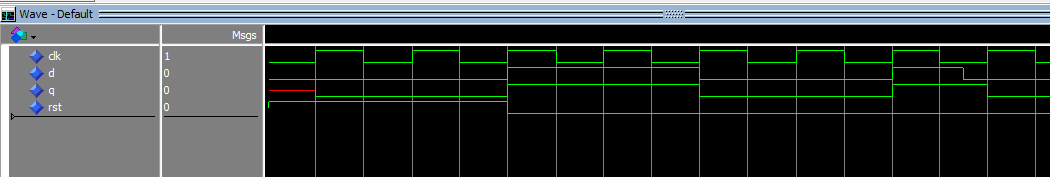
\includegraphics[width=0.8\textwidth]{Figs/tut_fig21.png}
	\end{figure}
\end{frame}





\end{document}
